% !TEX encoding = UTF-8
% !TEX TS-program = pdflatex
% !TEX root = ../tesi.tex

%**************************************************************
\chapter{Data analysis and the outcomes}
\label{cap:data-analysis}
This chapter illustrates the analysis of the collected data, enriched by discussions and experiments.
%**************************************************************
\section{Discussions, experiments and premises about collected data analysis}
Before discussing the obtained acceptability model and describing the "Zero-Effort Attack" tool, it is necessary to pin some premises and discuss some hot spots. Thus, some small experiments carried out are cited to show how the research field is very large and full of possible paths to take.

\subsection{Number of friend request}
\label{cap:number-friend-req}
First of all, a clarification about the number of friend requests.\\
According to the law of large numbers, with a greater amount of data collected, the result of the analyzed data is more certain and therefore more valid.\\\\Thus, is correct to affirm that \texttt{3} is a small number, but it was decided thinking about the smallest exhaustive number of friend requests to do considering the available time.\\A greater number would have led to a greater number of logins and friend requests, actions that could have led Facebook to block profiles.\\With more time, logins and friend requests would be spread over time, so as not to be blocked.\\\\So, \texttt{3} is the perfect number for this case of study (i.e. for the internship), because only one request not could be valued, 2 requests bring the analysis in a \textit{fifty-fifty} situation, with 3 requests one of the two possible results (friend request accepted or not) triumphs over the other.\\\\It's also important to underline that the result of \textbf{the analysis is preliminary}: with more requests (but anyway the number must be odd) the model of acceptance could undergo substantial changes.\\\\Also for this reason, during the development of all tools, it has always been born in mind that they must be implemented to work with a variable amount of data.
\subsection{\texttt{victims.json} dataset: why is it so unbalanced?}
\label{cap:discuss-dataset-victims}
After the first phase of data collection, it was possible to notice that most of the users on Facebook do not enter a lot of data in their profile, making the dataset of data collected immediately very unbalanced.\\More precisely, few users enter their age, city of residence, and occupation (many times it is present but blatantly bogus).\\Added to this is the fact that very few underage users who make it clear their age are very few (about 2 out of more than 1000 total profiles collected).\\In many cases, age can only be guessed by looking at the profile image, but this is not an evaluation criterion on which to reason.\\Thus, some categories contained a greater number of profiles and this caused the dataset to be very unbalanced.\\\\In the first place, it was decided that these profiles were categorized anyway, but for every category, the number of profiles examined is the same.\\The extra profiles were useful when it was necessary to replace some victim profiles that, for some reason, could no longer be considered.
\\\\Then, it was decided to remove the classes of the parameters that consider the minors, and the "\texttt{current\_town\_value}" and "\texttt{occupation\_value}" parameters.\\All three are interesting factors to analyze in future works (\ref{cap:future-works}).
\subsection{Profile picture: is it really so important?}
\label{cap:discuss-image-profile}
For this project, 12 attacking profiles were created, 6 of which with a real profile image, depicting a (non-existent) person.\\
The profile pictures were chosen consistently with the age that the corresponding attacker profile claimed to have.\\\\For example, the attacker profile "\texttt{PF-9}" is a 70-year-old woman and her profile picture of her represents a woman who could be said to be around that age. The value of the "\texttt{age\_range}" parameter of this profile is "\texttt{3}", as the age is greater than 50 years.\\In this range, however, there are also people of just 52 years and 20 years of difference are not exactly few if you wanted to make a comparison.\\The "PF-9" profile was not widely accepted, but how can one be sure that the same fate would have had a profile 20 years younger but still belonging to $\texttt{age\_value} = 3$?\\\\For this reason, they took some profiles with the real profile image and changed the profile image with one that, at first glance, showed a different age from the one declared (not too different of course).\\\\A note before showing the results: to make the change more consistent, the year of birth that the profile declares should also have been changed.\\With an extra profile used for testing of various kinds, this experiment was done, but Facebook took steps by blocking the profile.\\So, it was decided to change only the profile image, taking as good as stated in the chapter \ref{cap:alt-technology}, or that when a user receives the friend request he is easily influenced by the profile image, so much so that many times he does not even check the true age on the appropriate page.
\\\\The results are now illustrated:
\begin{center}
\begin{tabular}[c]{ |c|c|m{1.5cm}|m{1.5cm}|c| } 
	\hline
	\cellcolor[HTML]{b0d7ff}\textsc{cod} & 
	\cellcolor[HTML]{b0d7ff}\textsc{label} & 
	\multicolumn{1}{|c|}{\cellcolor[HTML]{b0d7ff}\textsc{old img}}&
	\multicolumn{1}{|c|}{\cellcolor[HTML]{b0d7ff}\textsc{new img}}&
	\cellcolor[HTML]{b0d7ff}\textsc{friend request accepted}\\
	%\cellcolor[HTML]{e6f2ff}
	\hline 
	\cellcolor[HTML]{b0d7ff}\texttt{PF-9}
	&\cellcolor[HTML]{e6f2ff}\texttt{FT3}
	&\vspace{.15cm}	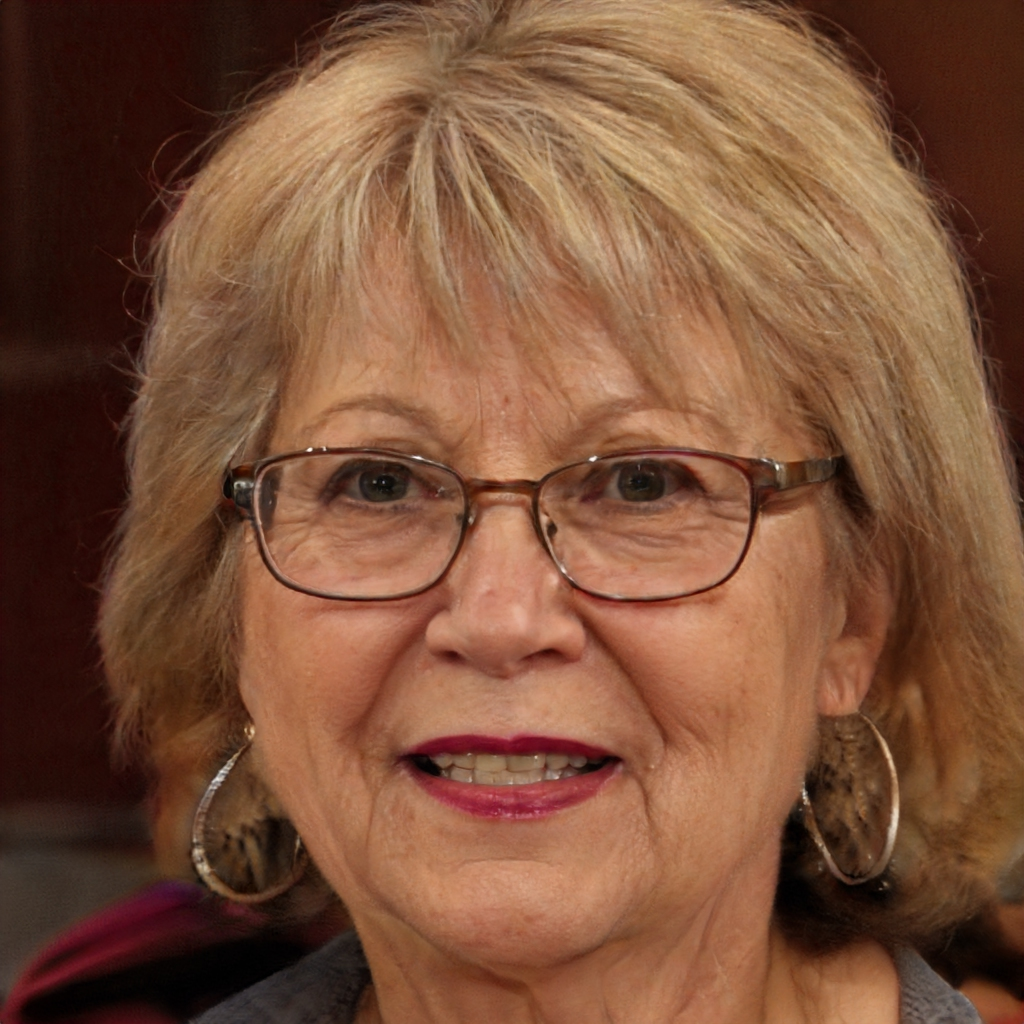
\includegraphics[height=1.5cm]{immagini/FT3.jpg}
	&\vspace{.15cm}	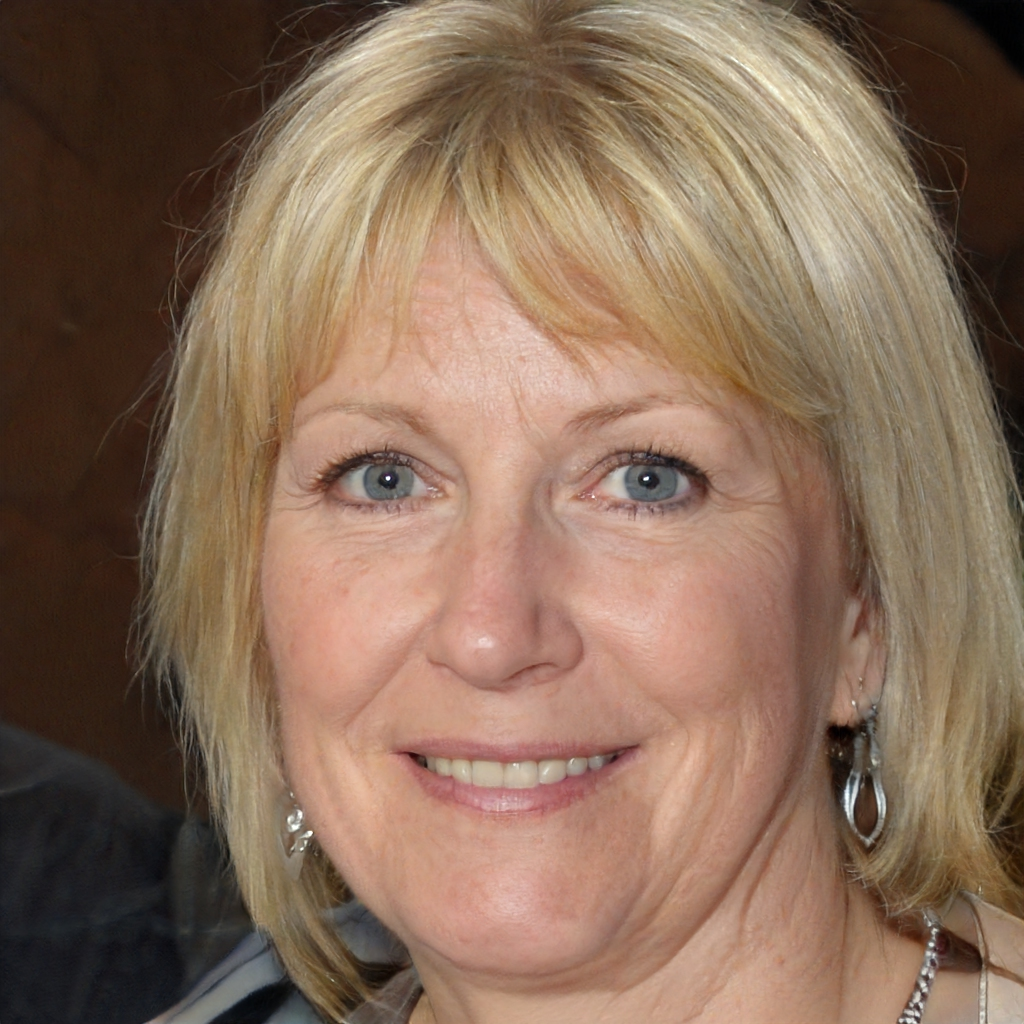
\includegraphics[height=1.5cm]{immagini/FT3-new.jpg}
	& +3 [\texttt{MT2}, \texttt{MT2}, \texttt{MT2}]\\	 
	\hline 		
	\cellcolor[HTML]{b0d7ff}\texttt{PF-5}
	&\cellcolor[HTML]{e6f2ff}\texttt{MT2}
	&\vspace{.15cm}	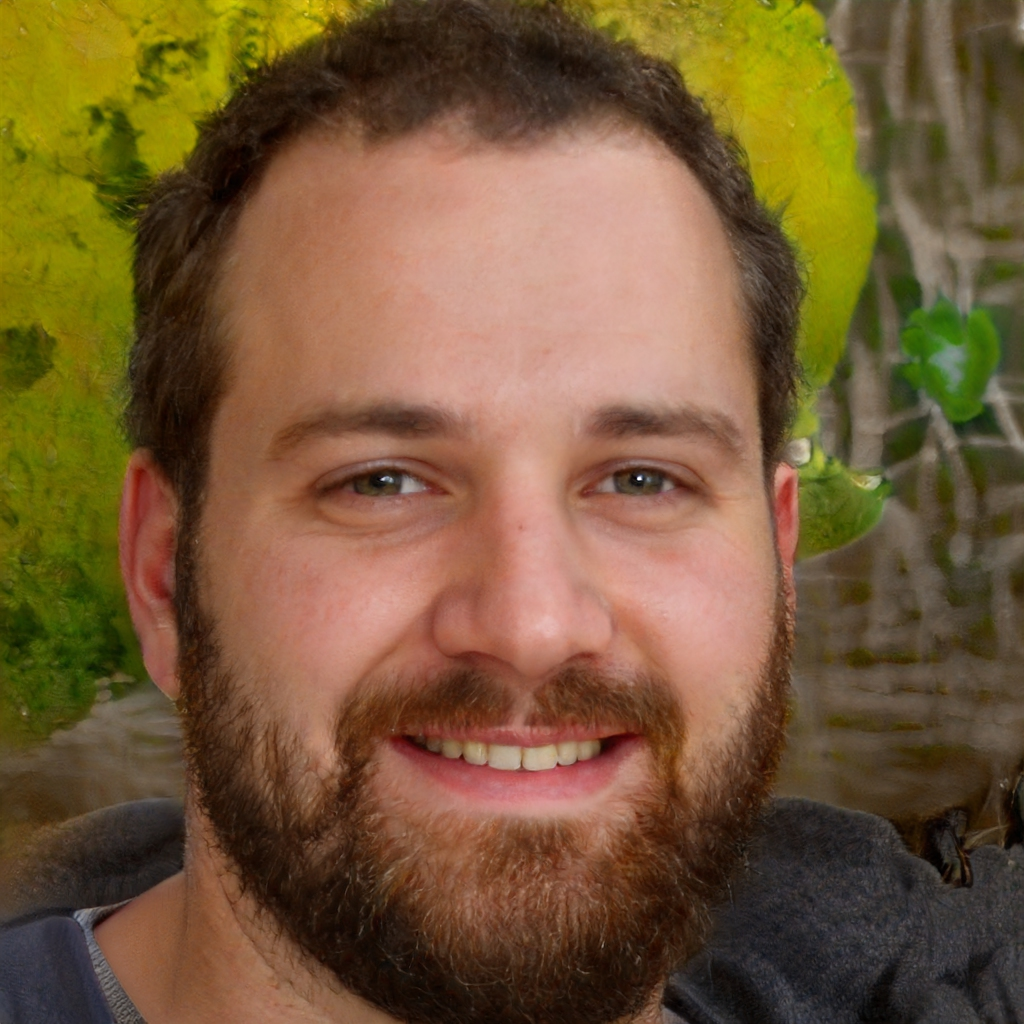
\includegraphics[height=1.5cm]{immagini/MT2.jpg}
	&\vspace{.15cm}	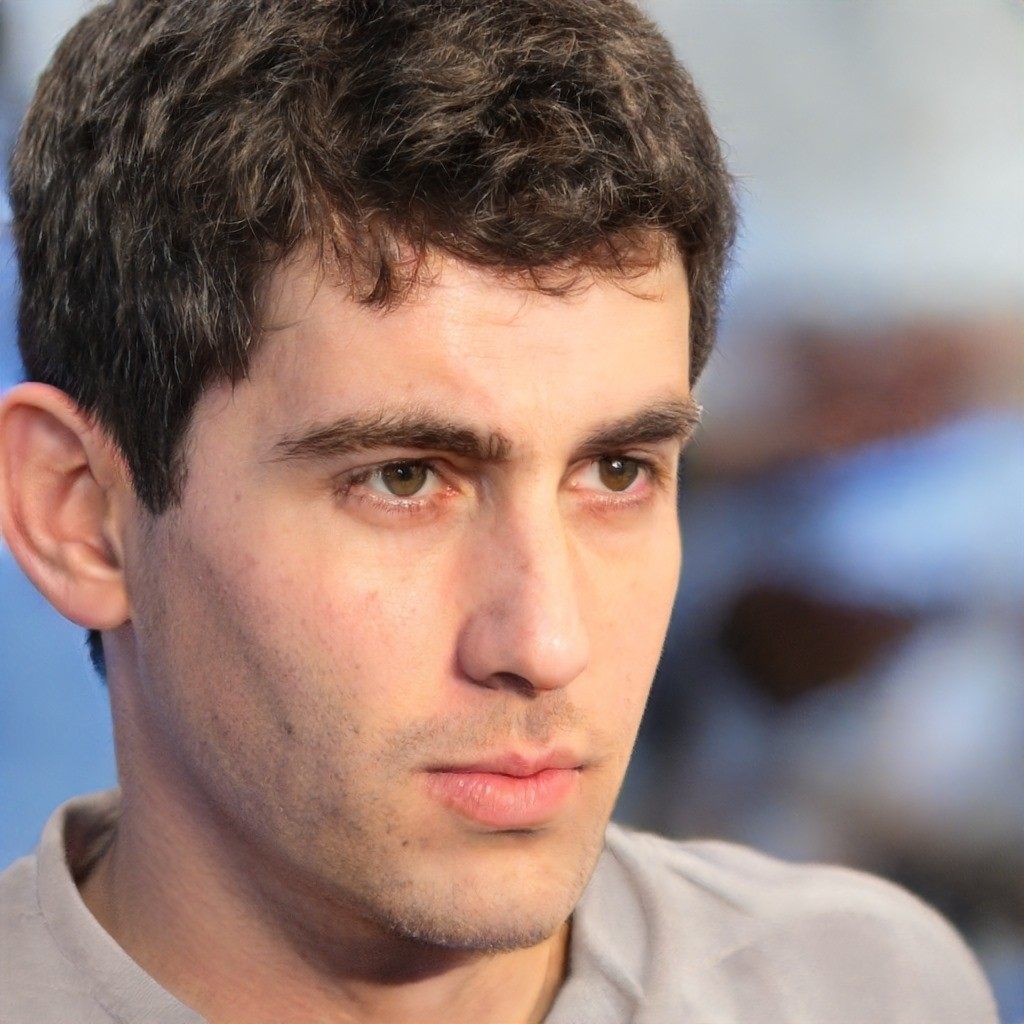
\includegraphics[height=1.5cm]{immagini/MT2-new.jpg}
	& +2 [\texttt{FT2}, \texttt{FT3}]\\	 
	\hline
	\cellcolor[HTML]{b0d7ff}\texttt{PF-3}
	&\cellcolor[HTML]{e6f2ff}\texttt{MT3}
	&\vspace{.15cm}	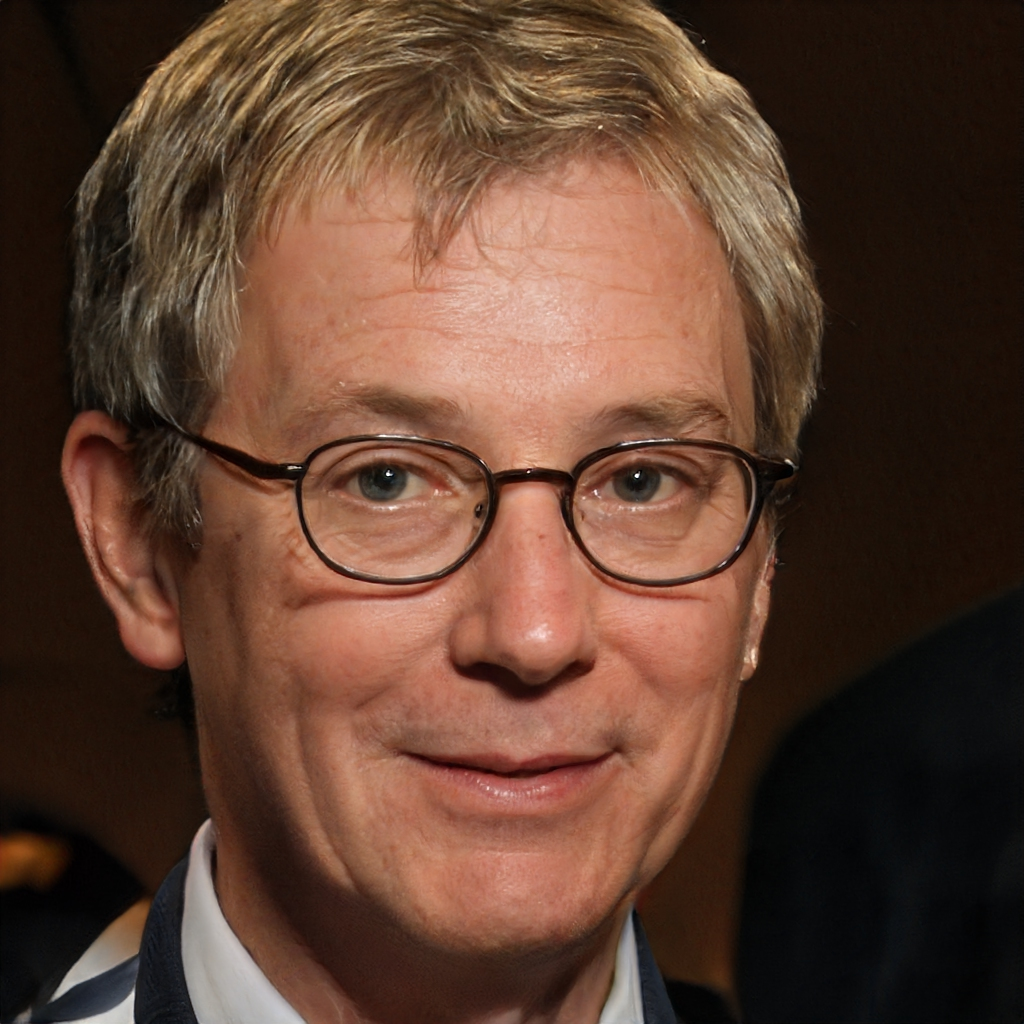
\includegraphics[height=1.5cm]{immagini/MT3.jpg}
	&\vspace{.15cm}	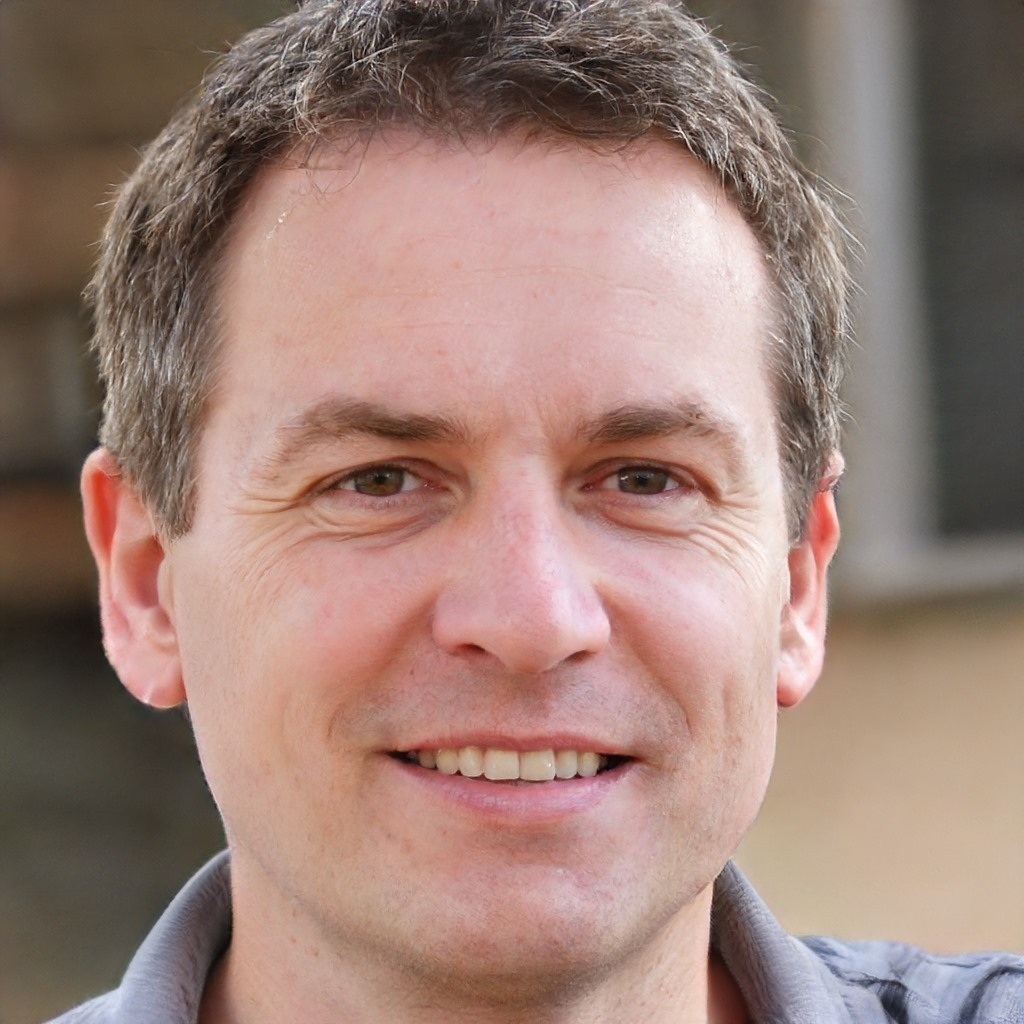
\includegraphics[height=1.5cm]{immagini/MT3-new.jpg}
	& +0 \\	 
	\hline
	\cellcolor[HTML]{b0d7ff}\texttt{PF-0}
	&\cellcolor[HTML]{e6f2ff}\texttt{MT4}
	&\vspace{.15cm}	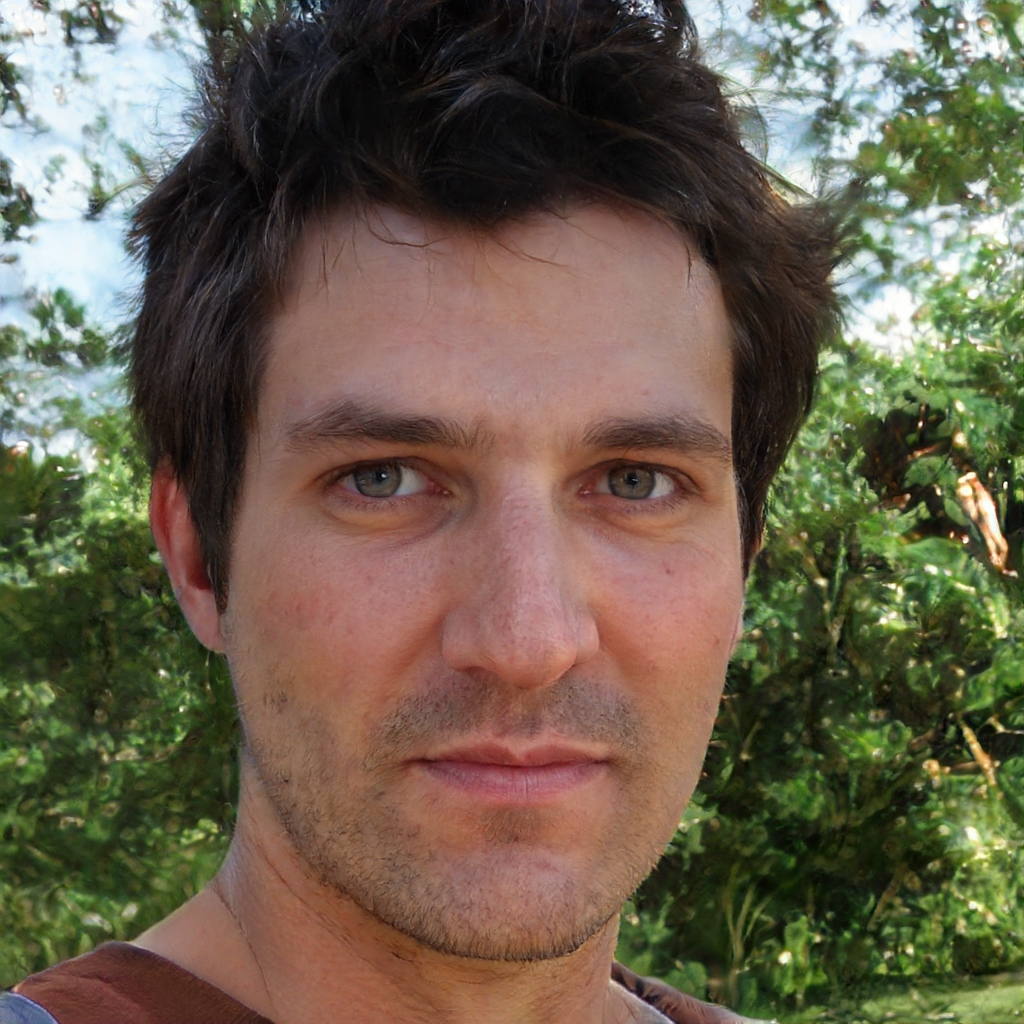
\includegraphics[height=1.5cm]{immagini/MT4.jpg}
	&\vspace{.15cm}	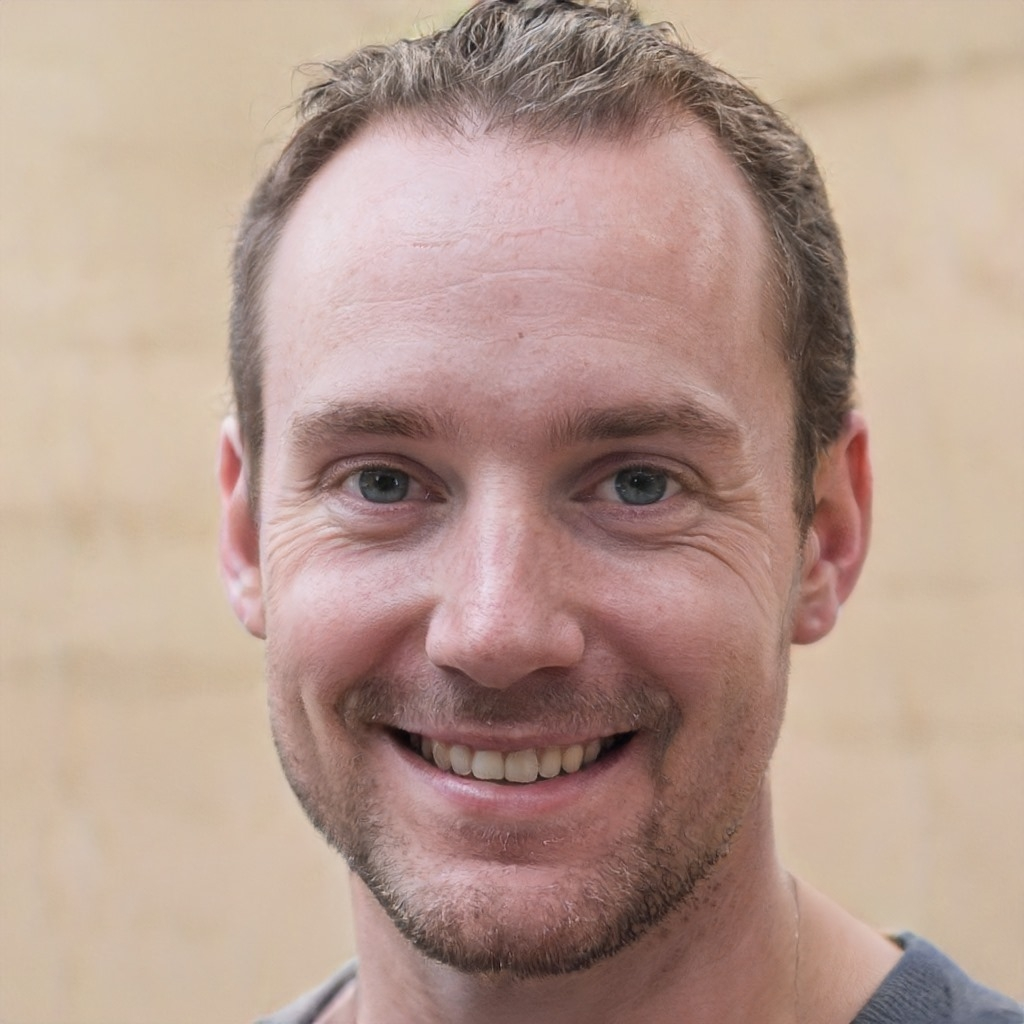
\includegraphics[height=1.5cm]{immagini/MT4-new.jpg}
	&+2 = [\texttt{FF3}, \texttt{FT3}]\\
	\hline 	 	 	 	 	
\end{tabular}
	
\end{center}
(A note: after changing his picture profile, \texttt{PF-5} received a friend request from a woman, the first one request for him)\\
The importance of the profile image is therefore a valid starting point on which to deepen with a dedicated case study.
\subsection{Unexpected situations}
\subsubsection*{Friend requests from an external profile to an attacker profile}
This is the most unexpected situation: the attacker profiles must only to send the friend request. In a sense, one could say that they would have to work in the shadows.\\However, some attacking profiles found themselves struggling with friend requests from other real profiles!\\It was decided to accept all friend requests to see the behavior that these profiles would then assume, but there is nothing relevant to report, except that some profiles have started sending many messages to these attacking profiles (details in the next chapter). Attackers who have received friend requests are reported to be: PF-0, PF-6, PF-7, PF-8, PF-9, and PF-11. In particular, the PF-6 and PF-11 profiles have really received many requests for friendship: analyzing them both are profiles of women, both have the real profile image and are young. The papers said that friend requests from women are more easily acceptable, but even that these profiles received so many requests, well, it was not imaginable!
\subsubsection*{Victim profiles wrote messages to (female) attacker profiles, but not with so good intentions}
Facebook is a platform where people can meet and start a conversation.\\Well, it was assumed that some victim profiles could accept the friendship and then write messages, to understand if they really know each other in reality or even just to make new acquaintances. The thing that was not at all expected was the number of messages received. \\The profiles of the attackers who received messages are all women involved in this project: \texttt{PF-6, PF-7, PF-8, PF-9, PF-10, PF-11}. Those who have received the most crops are \texttt{PF-6, PF-9, PF-11}. All these profiles received many messages only and exclusively from men.Many of these continued to write insistently even though they received no response.\\\\
\quad \textit{An example of a message that }\texttt{PF-10}\textit{ received:}\\
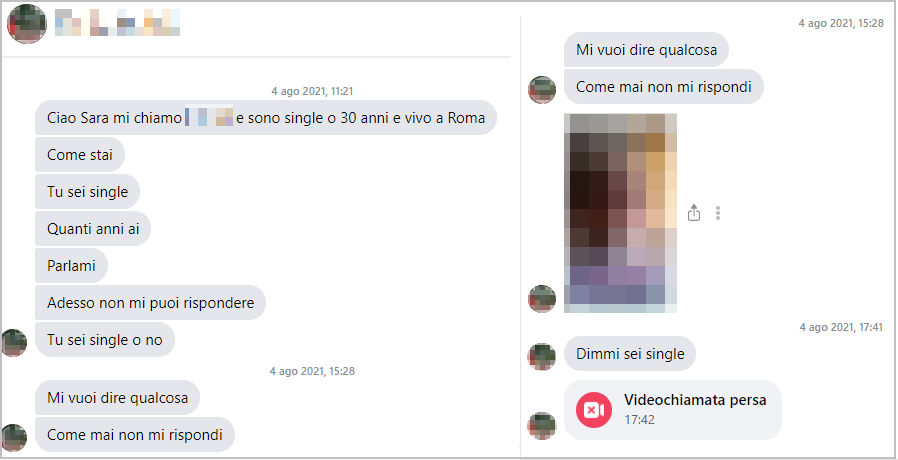
\includegraphics[height=6cm]{immagini/pf-10.png}\\\\
\quad \textit{An example of a message that }\texttt{PF-9}\textit{ received:}\\
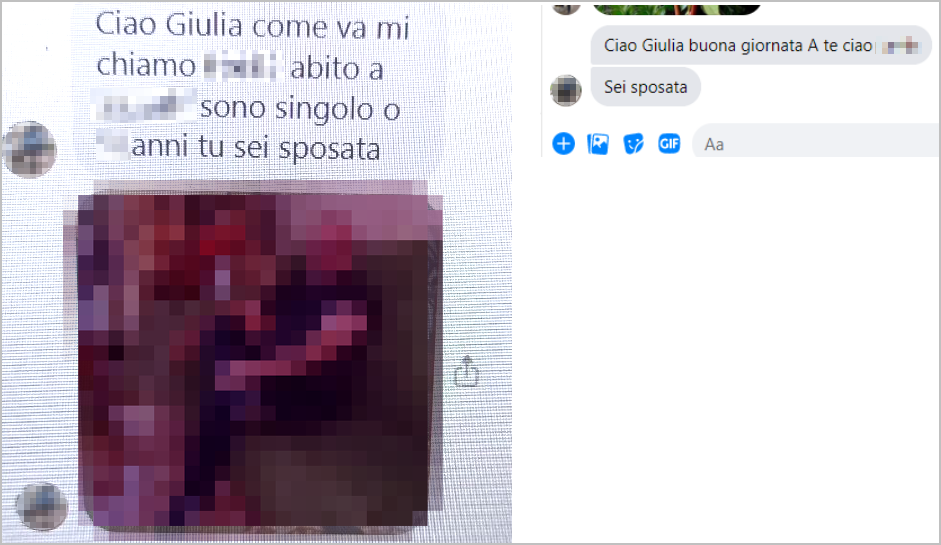
\includegraphics[height=6cm]{immagini/pf-9.png}
\textit{\\(A few days later, this first message was then deleted (leaving only the photo) and replaced with the messages shown on the right).}\newpage
\quad \textit{An example of a message that }\texttt{PF-11}\textit{ received:}\\

\includegraphics[height=5cm]{immagini/pf-11.png}
\textit{\\(This is an example of a tireless profile: despite having received no response, he still continues to text almost daily).}
\subsubsection*{A profile removed an attacker profile from friends}
\label{cap:discuss-removed-friends}
In short, a "\texttt{MT3}" victim profile removed the "\texttt{PF-8}" attacker profile from his friends list a few days after accepting his friend request.\\ 
This situation was unexpected in the first place, but, thinking about it, it is not so strange.\\As some papers said, there are some people that check very carefully the person who sent them the friend request: sometimes, first, they check the profile to decide if accept the friend request; other times, first they accept the friend request and then check the profile, in order to remove it from the friends if there are some characteristics that the person doesn't like.\\
Probably the profile more empty than usual (it is a fake profile where not a lot of content has been shared) and with a not real profile picture, made the victim suspicious, so much so as to remove this profile from the friend's list.
\section{Model of acceptance}
\label{cap:model-of-acceptance}
With a tool, called \texttt{acceptance\_model.py}, which analize the content of \\ \texttt{distribution\_update.json} dataset (details in \ref{cap:distribution-update}), an acceptance model will be created.\\
The tool, run from the terminal, requires the \texttt{distribution\_update.json} dataset and for each type of victim, it describes the acceptance rate of every type of attacker profile. Considering that the number of friend requests from an attacker profile to each type of victim profile is "3", an attacker profile could have 4 types of percentual, based on the number of how many friends request that type of victim have accepted:
\begin{itemize}
	\item \texttt{1\%} if the acceptance rate is \texttt{0/3}; \\(It was decided to put 1\% instead of 0\% because there can always be an exception);
	\item \texttt{33\%} if the acceptance rate is \texttt{1/3};
	\item \texttt{66\%} if the acceptance rate is \texttt{2/3};
	\item \texttt{99\%} if the acceptance rate is \texttt{3/3};	\\(It was decided to put 99\% instead of 100\% because there can always be an exception).
\end{itemize}
The tool does a sum of percentages for each type of victim for each type of attacking profile, creating the model of acceptance that is now shown:
\begin{center}
	\label{cap:table-model-acceptance}
	\begin{tabular}{|c|l|}
		\toprule
		\cellcolor[HTML]{b0d7ff}\textbf{VICTIM} & 
		\cellcolor[HTML]{b0d7ff}\textbf{ACCEPTANCE RATE}
		\\ 
		\midrule
		\multirow{2}*{\textbf{FT2}} 
		& \cellcolor[HTML]{e6f2ff}with $\approx 33\%$\quad$\to$ \texttt{MT4, MT2, FT4, FF3, FT2}\\			
		& with $\approx 1\%$\quad$\>\>\to$ \texttt{MF4, MF2, MT3, MF3, FF4, FF2, FT3}\\
		\midrule
		
		\multirow{3}*{\textbf{FT3}} 
		& \cellcolor[HTML]{e6f2ff}with $\approx 66\%$\quad$\to$ \texttt{MT3, FT4}\\		
		& with $\approx 33\%$\quad$\to$ \texttt{MT4, MF4, MT2, FF4, FT2}\\
		& with $\approx 1\%$\quad$\>\>\to$ \texttt{MF2, MF3, FF2, FT3, FF3}\\
		\midrule
		
		\multirow{3}*{\textbf{FT4}} 
		& \cellcolor[HTML]{e6f2ff}with $\approx 66\%$\quad$\to$ \texttt{MT4, FT4}\\		
		& with $\approx 33\%$\quad$\to$ \texttt{MF4, FT3, FF3, FT2}\\
		& with $\approx 1\%$\quad$\>\>\to$ \texttt{MF2, MT3, MF3, MT2, FF4, FF2}\\
		\midrule
		
		\multirow{3}*{\textbf{FF2}}
		& \cellcolor[HTML]{e6f2ff}with $\approx 66\%$\quad$\to$ \texttt{FT4}\\		
		& with $\approx 33\%$\quad$\to$ \texttt{MF2, FF2, FT3}\\
		& with $\approx 1\%$\quad$\>\>\to$ \texttt{MT4, MF4, MT3, MF3, MT2, FF4, FF3, FT2}\\
		\midrule
		
		\multirow{3}*{\textbf{FF3}} 
		& \cellcolor[HTML]{e6f2ff}with $\approx 66\%$\quad$\to$ \texttt{MT4, FT2}\\		
		& with $\approx 33\%$\quad$\to$ \texttt{MT3, FF3}\\
		& with $\approx 1\%$\quad$\>\>\to$ \texttt{MF4, MF2, MF3, MT2, FT4, FF4, FF2, FT3}\\
		\midrule
		
		\multirow{2}*{\textbf{FF4}} 
		& \cellcolor[HTML]{e6f2ff}with $\approx 33\%$\quad$\to$ \texttt{FT2}\\
		& with $\approx 1\%$\quad$\>\>\to$ \texttt{MT4, MF4, MF2, MT3, MF3, MT2, FT4, FF4, FF2, FT3, FF3}\\
		\midrule
		
		%----------------------------------------------------------------%
		
		\multirow{4}*{\textbf{MT2}} 
		&\cellcolor[HTML]{e6f2ff} with $\approx 99\%$\quad$\to$ \texttt{MT2, FT4}\\
		& with $\approx 33\%$\quad$\to$ \texttt{FT3, FT2}\\
		& with $\approx 33\%$\quad$\to$ \texttt{MF4, MF2, MT3, FF2}\\
		& with $\approx 1\%$\quad$\>\>\to$ \texttt{MT4, MF3, FF4, FF3}\\
		\midrule
		
		\multirow{2}*{\textbf{MT3}}
		&\cellcolor[HTML]{e6f2ff} with $\approx 66\%$\quad$\to$ \texttt{MT4, MT2, FT4, FF4, FF2, FT3}\\
		& with $\approx 33\%$\quad$\to$ \texttt{MF4, MF2, MT3, MF3, FF3, FT2}\\
		\midrule
		
		\multirow{4}*{\textbf{MT4}} 
		& \cellcolor[HTML]{e6f2ff}with $\approx 99\%$\quad$\to$ \texttt{FF2}\\
		& with $\approx 33\%$\quad$\to$ \texttt{MT4, MT2, FT4, FF3}\\
		& with $\approx 33\%$\quad$\to$ \texttt{MF4, MF2, MT3, FF4, FT3, FT2}\\
		& with $\approx 1\%$\quad$\>\>\to$ \texttt{MF3}\\
		\midrule
		
		\multirow{3}*{\textbf{MF2}} 
		& \cellcolor[HTML]{e6f2ff}with $\approx 66\%$\quad$\to$ \texttt{MT4}\\		
		& with $\approx 33\%$\quad$\to$ \texttt{MF4, MT2, FT4, FF2, FT2}\\
		& with $\approx 1\%$\quad$\>\>\to$ \texttt{MF2, MT3, MF3, FF4, FT3, FF3}\\
		\midrule
		
		\multirow{3}*{\textbf{MF3}} 
		& \cellcolor[HTML]{e6f2ff}with $\approx 66\%$\quad$\to$ \texttt{MF2, FT3, FT2}\\		
		& with $\approx 33\%$\quad$\to$ \texttt{MT4, MT3, MT2}\\
		& with $\approx 1\%$\quad$\>\>\to$ \texttt{MF4, MF3, FT4, FF4, FF2, FF3}\\
		\midrule
		
		\multirow{4}*{\textbf{MF4}} 
		& \cellcolor[HTML]{e6f2ff}with $\approx 99\%$\quad$\to$ \texttt{FT4}\\
		& with $\approx 33\%$\quad$\to$ \texttt{FT2}\\
		& with $\approx 33\%$\quad$\to$ \texttt{MT4, MF4, MF3, MT2, FF4, FF2, FF3}\\
		& with $\approx 1\%$\quad$\>\>\to$ \texttt{MF2, MT3, FT3}\\
		\bottomrule
		
		
	\end{tabular}	
\end{center}
\newpage
\section{Zero-Effort Attack}
\label{cap:zero-effort-attack}
\texttt{Zero-Effort Attack} is the name of the final tool. This was the goal of the internship. Its name is derived from the effective effort that the attacker gonna do, i.e. \texttt{zero}. That's because the attacker must put the URL of the victim profile on the terminal and the tool will show in the output the model of acceptance (chapter \ref{cap:table-model-acceptance}) for that type of victim.\\In detail, the tool, run from the terminal, requires as input:
\begin{itemize}
	\item \texttt{email},\\the email that the attacker use to log into Facebook.\\Accepted values: string parameter (\texttt{string});
	
	\item \texttt{pwd},\\the password that the attacker use to log into Facebook.\\Accepted values: string parameter (\texttt{string});
	
	\item \texttt{url},\\the URL of victim profile to attack.\\Accepted values: string parameter (\texttt{string});
\end{itemize}
This tool get the \texttt{email} and \texttt{password} parameters to log into Facebook.\\After that, it goes to the page of the victim profile thanks to the \texttt{URL} parameter.
Now the tool can be analize the victim, and the procedure is the same of the \texttt{classificator-profile} tool (chapter \ref{cap:classificator-profiles}).
\\Once the victim's profile has been analyzed, it categorizes it by assigning it the corresponding label.\\
With that label, the tool will examine the acceptance model and show in the terminal which type of attacker profiles are accepted and with what probability, to allow the attacker to create the best profile.
\\\\The image below display what the terminal show in the output to the attacker in the end of the procedure.\\\\
\begin{center}
	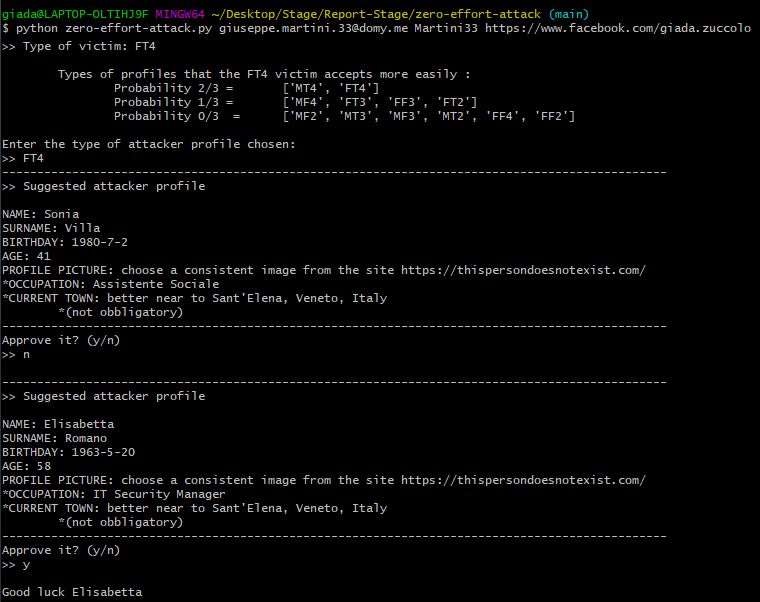
\includegraphics[height=3cm]{immagini/zero-effort-exe.png}
\end{center}